\documentclass[12pt]{article}
\usepackage[margin=1in]{geometry}
\usepackage[utf8]{inputenc}
\usepackage[T1]{fontenc}
\usepackage{graphicx}
\usepackage{booktabs}
\usepackage{amsmath}

\title{AIS Project}
\author{Juan Espinoza, Jianxiong Zheng, Ramsey To, Ulisse Palmiero}
\date{April 2026}

\begin{document}
\maketitle

We believe we should not move forward with the proposed strategy as a standalone active strategy.

The long-short momentum strategy shows some attractive features, especially its very low correlation
with the market and its positive annualized return of 3.36%. The annualized volatility is 9.50%,
producing a Sharpe ratio of 0.3540. However, this level of risk-adjusted performance is not strong
enough to justify full implementation, especially given the strategy’s downside risk. The maximum
drawdown is -31.72%, beginning in May 2008, and the recovery period is 150 months, which indicates
that investors may need to tolerate a very long period of underperformance.

The regression results also weaken the investment case. In the single-factor model, the strategy appears
to have a positive monthly alpha of 0.2815% with a statistically significant p-value of 0.0136, while its
market beta is almost zero. However, once we control for additional factors using the Carhart model,
the alpha becomes economically small and statistically insignificant. The intercept is -0.0145% per
month with a p-value of 0.8593, while the UMD coefficient is large and highly significant. This suggests
that the strategy’s returns are mainly explained by exposure to the momentum factor rather than by
unique alpha generation.

Although the strategy can provide diversification benefits when combined with the market portfolio, we
do not recommend moving forward with it as proposed. Achieving a 12% volatility target would require
126.30% exposure on both the long and short sides, resulting in 252.59% gross leverage. This creates
meaningful implementation risk, and transaction costs, shorting costs, and turnover would likely reduce
realized returns. Therefore, we would only consider this strategy as a small diversifying allocation after
further testing on trading costs, capacity, and risk controls.

% Auto-generated by ais_project.py -- do not edit manually

\section{Q1: Long-Short Portfolio Construction}

\begin{verbatim}
  High return (Jan 1975): 0.1597125
  Low  return (Jan 1975): 0.1807875

  First 12 months of Long-Short returns:
  Date  High_Return  Low_Return  LS_Return
197501    0.1597125   0.1807875 -0.0210750
197502    0.0532875   0.0525125  0.0007750
197503    0.0492625   0.0649375 -0.0156750
197504    0.0629125   0.0419750  0.0209375
197505    0.0406625   0.0504000 -0.0097375
197506    0.0626250   0.0580875  0.0045375
197507   -0.0462625  -0.0614500  0.0151875
197508   -0.0313625  -0.0127500 -0.0186125
197509   -0.0278625  -0.0459500  0.0180875
197510    0.0490625   0.0592875 -0.0102250
197511    0.0340125   0.0235375  0.0104750
197512   -0.0061250  -0.0073000  0.0011750
\end{verbatim}

\section{Q2: Annualized Performance}

\begin{verbatim}
  Annualized Mean Return : 0.0338 (3.38%)
  Annualized Std Dev     : 0.0950 (9.50%)
  Sharpe Ratio           : 0.3560
\end{verbatim}

\section{Q3: Maximum Drawdown}

\begin{verbatim}
  Max Drawdown           : -0.3172 (-31.72%)
  Drawdown Start (Peak)  : 200806
  Trough                 : 201202
  Recovery Date          : 202012
  Months to Recover      : 150
\end{verbatim}

\section{Q4: Leverage for 12\% Volatility Target}

\begin{verbatim}
  Current Ann. Volatility: 9.50%
  Scale Factor           : 1.2630
  Required Leverage      : 2.5260x
  (Each side weight      : 1.2630)
\end{verbatim}

\section{Q5: Single-Factor Regression}

\begin{verbatim}
                            OLS Regression Results                            
==============================================================================
Dep. Variable:                      y   R-squared:                       0.000
Model:                            OLS   Adj. R-squared:                 -0.002
Method:                 Least Squares   F-statistic:                  0.003065
Date:                Wed, 29 Apr 2026   Prob (F-statistic):              0.956
Time:                        22:32:57   Log-Likelihood:                 1306.9
No. Observations:                 600   AIC:                            -2610.
Df Residuals:                     598   BIC:                            -2601.
Df Model:                           1                                         
Covariance Type:            nonrobust                                         
==============================================================================
                 coef    std err          t      P>|t|      [0.025      0.975]
------------------------------------------------------------------------------
const          0.0028      0.001      2.491      0.013       0.001       0.005
mktrf         -0.0014      0.025     -0.055      0.956      -0.050       0.047
==============================================================================
Omnibus:                       34.322   Durbin-Watson:                   1.864
Prob(Omnibus):                  0.000   Jarque-Bera (JB):               74.836
Skew:                          -0.320   Prob(JB):                     5.62e-17
Kurtosis:                       4.607   Cond. No.                         22.2
==============================================================================

Notes:
[1] Standard Errors assume that the covariance matrix of the errors is correctly specified.
  Idiosyncratic Vol (sigma_e) monthly: 0.027450
  Idiosyncratic Vol (sigma_e) annual : 0.095090
\end{verbatim}

\section{Q6: Optimal Two-Asset Portfolio}

\begin{verbatim}
  Optimal Weight in LS Strategy : 1.0302
  Optimal Weight in Market Port.: -0.0302
  (Inputs: alpha=0.002829, sigma_e^2=0.000754,
   mean_mktrf=0.007423, var_mktrf=0.002037)
\end{verbatim}

\section{Q7: Factor Correlations}

\begin{verbatim}
  corr(LS, MKTRF) : -0.0023
  corr(LS, SMB  ) : 0.0841
  corr(LS, HML  ) : -0.1949
  corr(LS, UMD  ) : 0.7013
\end{verbatim}

\section{Q8: Multi-Factor Regressions}

\begin{verbatim}
Fama-French 3-Factor Model (LS ~ mktrf + smb + hml)
                            OLS Regression Results                            
==============================================================================
Dep. Variable:                      y   R-squared:                       0.044
Model:                            OLS   Adj. R-squared:                  0.039
Method:                 Least Squares   F-statistic:                     9.145
Date:                Wed, 29 Apr 2026   Prob (F-statistic):           6.35e-06
Time:                        22:32:57   Log-Likelihood:                 1320.4
No. Observations:                 600   AIC:                            -2633.
Df Residuals:                     596   BIC:                            -2615.
Df Model:                           3                                         
Covariance Type:            nonrobust                                         
==============================================================================
                 coef    std err          t      P>|t|      [0.025      0.975]
------------------------------------------------------------------------------
const          0.0034      0.001      3.008      0.003       0.001       0.006
mktrf         -0.0340      0.026     -1.334      0.183      -0.084       0.016
smb            0.0641      0.038      1.687      0.092      -0.011       0.139
hml           -0.1721      0.036     -4.756      0.000      -0.243      -0.101
==============================================================================
Omnibus:                       35.102   Durbin-Watson:                   1.870
Prob(Omnibus):                  0.000   Jarque-Bera (JB):               64.109
Skew:                          -0.390   Prob(JB):                     1.20e-14
Kurtosis:                       4.398   Cond. No.                         35.9
==============================================================================

Notes:
[1] Standard Errors assume that the covariance matrix of the errors is correctly specified.

Carhart 4-Factor Model (LS ~ mktrf + smb + hml + umd)
                            OLS Regression Results                            
==============================================================================
Dep. Variable:                      y   R-squared:                       0.508
Model:                            OLS   Adj. R-squared:                  0.504
Method:                 Least Squares   F-statistic:                     153.5
Date:                Wed, 29 Apr 2026   Prob (F-statistic):           3.95e-90
Time:                        22:32:57   Log-Likelihood:                 1519.5
No. Observations:                 600   AIC:                            -3029.
Df Residuals:                     595   BIC:                            -3007.
Df Model:                           4                                         
Covariance Type:            nonrobust                                         
==============================================================================
                 coef    std err          t      P>|t|      [0.025      0.975]
------------------------------------------------------------------------------
const         -0.0001      0.001     -0.154      0.878      -0.002       0.001
mktrf          0.0567      0.019      3.029      0.003       0.020       0.093
smb            0.0553      0.027      2.028      0.043       0.002       0.109
hml           -0.0096      0.027     -0.356      0.722      -0.062       0.043
umd            0.4524      0.019     23.678      0.000       0.415       0.490
==============================================================================
Omnibus:                       15.007   Durbin-Watson:                   1.987
Prob(Omnibus):                  0.001   Jarque-Bera (JB):               29.254
Skew:                          -0.058   Prob(JB):                     4.44e-07
Kurtosis:                       4.075   Cond. No.                         36.4
==============================================================================

Notes:
[1] Standard Errors assume that the covariance matrix of the errors is correctly specified.

Model Choice: Carhart 4-Factor is used to assess incremental alpha.
Rationale: UMD captures single-stock momentum; controlling for it isolates
the alpha that is purely due to industry-level momentum, not stock-level.
\end{verbatim}

\begin{figure}[htbp]
    \centering
    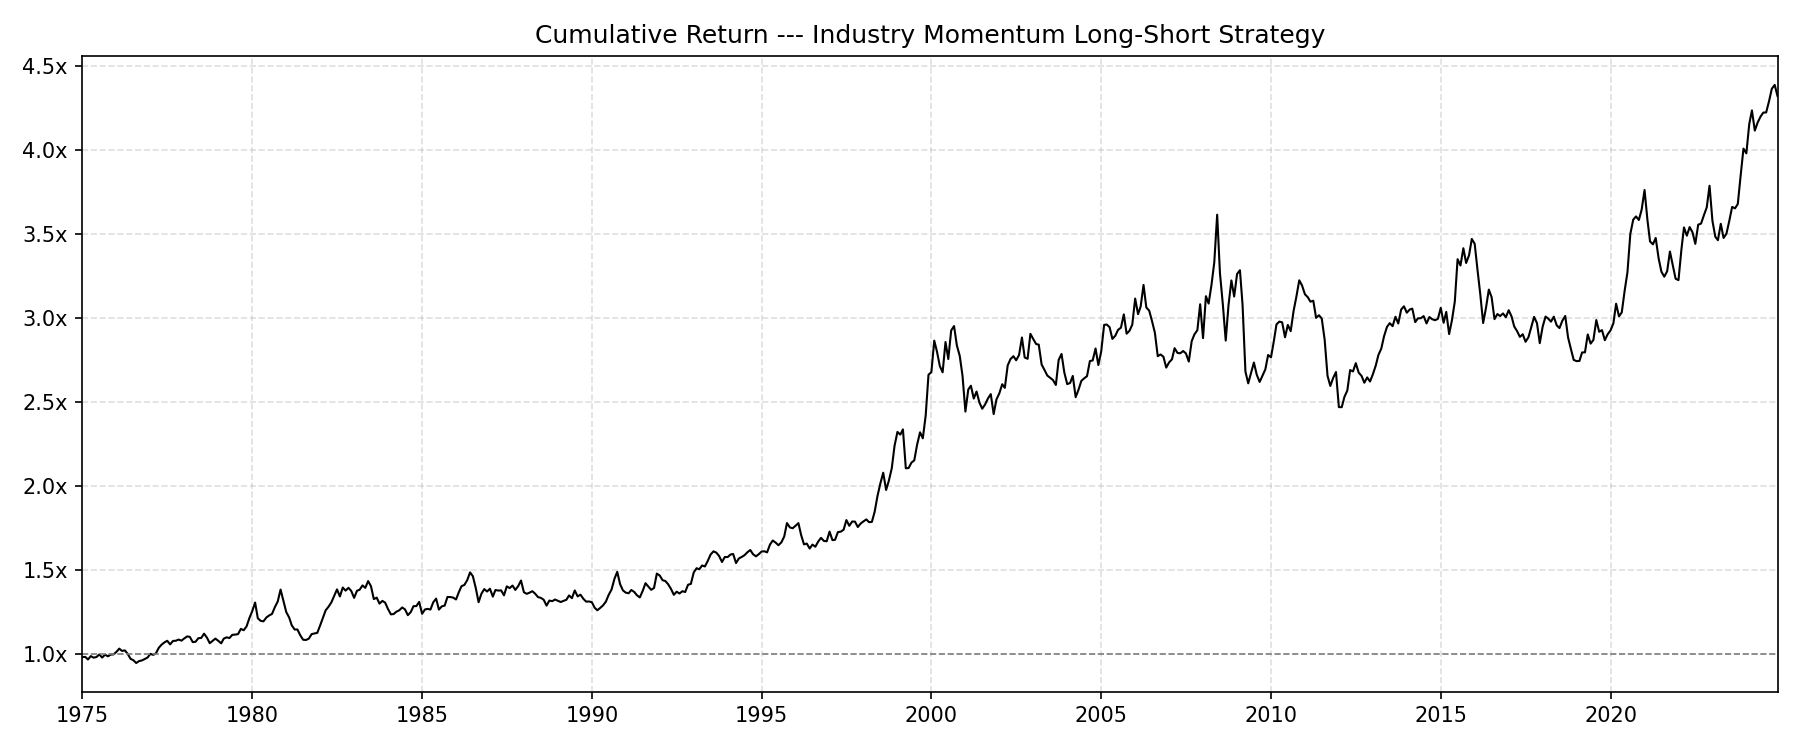
\includegraphics[width=\linewidth]{cumret_chart.png}
    \caption{Cumulative Return --- Industry Momentum Long-Short Strategy}
\end{figure}

\begin{figure}[htbp]
    \centering
    
\includegraphics[width=\linewidth]{drawdown_chart.png}
    \caption{Drawdown --- Industry Momentum Long-Short Strategy}
\end{figure}


\end{document}
